

%	Target..: Scalable Tools Workshop (2015)
%	Due.....: September 2nd

\documentclass{acmtog}
\excludecomment
%   Removed for ACM style guide compliance:
%
%\usepackage[utf8]{inputenc}
%\usepackage{amsmath}
%\usepackage{amsfonts}
%\usepackage{amssymb}
%\usepackage{graphicx}

\title{DESIGN and IMPLEMENTATION of\\
	SOS: Scalable Observation System\\
	\hrulefill\\
	[1em]Observation, Introspection, and Awareness for\\Distributed Scientific Work Flows at Scale\\}
\author{
        Chad Wood
		\affil{    
	    Department of Computer Science
	    University of Oregon
	    Eugene, OR 97403-1202 USA
	    }
        \and
        Daniel Ellsworth
		\affil{    
	    Department of Computer Science
	    University of Oregon
	    Eugene, OR 97403-1202 USA
	    }
        \and
        Allen Malony\\
		\affil{    
	    Department of Computer Science
	    University of Oregon
	    Eugene, OR 97403-1202 USA
	    }
}
\date{\today}

\begin{document}
\markboth{Author Name}{Article Title}
\maketitle
\begin{abstract}
The SOS project implements a distributed runtime tool-kit purposed with providing  observation, introspection, and awareness across heterogeneous systems in exascale HPC environments.  In addition to the development of software artifacts, this project contributes descriptions of the essential structures, patterns, and information flow required to facilitate effective dynamic system control, self-description, and data stores able to provide useful information from a variety of perspectives.
\end{abstract}

\keywords{Scientific Work Flows, HPC, Monitoring, Optimization, Self-Tuning}
\newpage
\tableofcontents
\newpage


\section{Introduction}\label{introduction}
\subsection{Purpose}
\paragraph{}Present day HPC environments impose varied and acute  design constraints on the applications they host, limiting the ability of complex heterogeneous tasks to coordinate their action, introspection, and control with a common framework, spanning local and global scopes.  Scientific work flows often are data-driven (dynamic) across their entire life cycle, and consequently it is unproductive to Engaging this challenging environment, the SOS project represents an effort to develop analytical models enunciating useful constraints and principles for coordinating scientific work flows.  Along with basic research, practical software tools will be created for integration into existing HPC projects.
\subsection{Motivation}
\paragraph{}Some motivating notions.
\subsection{Design Map}
\paragraph{}
\section{Design Considerations}
\subsection{Work Flows and Performance}
\subsection{The View From Nowhere}
\paragraph{}The 'central' point of view of the functioning of an exascale system is anywhere you decide to look.
\subsection{Risks and Volatile Areas}
\subsection{HPC Libraries as Input}
\section{Architecture}
\subsection{Overview}
\paragraph{}SOS is implemented primarily in ANSI standard C as a library of functions, data structures, and a run-time daemon.  SOS also features a centralized data store built with one of several SQL server solutions, or a write-only .CSV 'dump' for highly-constrained work flow execution environments that do not support heterogeneous application launches.
\paragraph{LIBRARY}
\paragraph{DATA STRUCTURES}
\paragraph{DAEMON}
\paragraph{DATABASE}
\section{High Level Design}
\subsection{Some Component Title}
\subsection{Some OTHER Component Title}
\section{Low Level Design}
\subsection{Some Implementation Detail}
\subsection{Some OTHER Implementation Detail}
\section{Experiments and Results}
\subsection{Some Experiment}
\subsection{Some Other Experiment}
\subsection{Recommendations}
\section{Conclusion}
\subsection{Summary of Efforts}
\subsection{Lessons Learned}
\subsection{Planned Future Work}
\paragraph{}
\begin{figure}
\centering
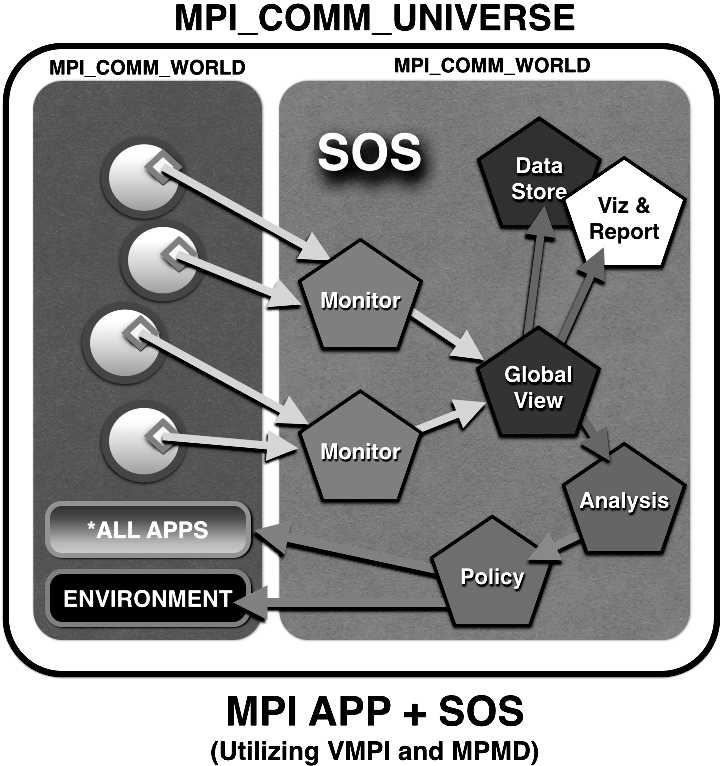
\includegraphics[width=0.7\linewidth]{./sos-overview-2}
\caption[Figure 1: SOS]{An image as an example.}
\label{fig:sos-overview.png}
\end{figure}
\begin{itemize}
\item{An example of a list.}
\item{Another item in that list.}
\end{itemize}
\newpage
\nocite{*}
\bibliographystyle{abbrv}
\bibliography{drp-contract-proposal.bib}
\end{document}
%EOF